\documentclass[11pt]{article}
\usepackage[margin=1in]{geometry}
\usepackage{graphicx,booktabs,amsmath,siunitx,microtype}
\usepackage[colorlinks=true,allcolors=blue]{hyperref}

\title{Which constitutive model do measured cavitation records prefer?}
\author{PyIMR}
\date{\today}

\begin{document}
\maketitle

\begin{abstract}
We compare seventeen constitutive models against laser-induced cavitation records in
gelatin at three temperatures, using Bayesian model selection with a noise scale measured
from trial-to-trial spread and a prior that prices a model down where it merely reproduces
a simpler one it contains. A quadratic Zener solid --- strain-stiffening elasticity
\emph{and} stress relaxation --- wins at every temperature, reaching a residual of
$\chi^2/N = 1.23$ to $1.35$ against experimental repeatability. Neither ingredient
suffices alone: relaxation without stiffening reaches $1.41$ to $2.94$, and every
memoryless model lands above $12$. The advantage of the stiffening term collapses as the
gel warms, which is the clearest physical signal in the comparison. We report the
limitations plainly: the reported residuals are ceilings rather than estimates, because
the winning model's best-fitting region is partly unintegrable.
\end{abstract}

\section{Setup}

Each dataset is a set of repeated laser-induced cavitation events at one temperature,
recorded as $R(t)/R_{\max}$. Figure~\ref{fig:records} shows the mean trace and the
trial-to-trial spread, which is what we use as the measurement noise: it is measured
rather than assumed, so a residual of $\chi^2/N \approx 1$ means a model reproduces the
record to within experimental repeatability.

\begin{figure}[htbp]
\centering
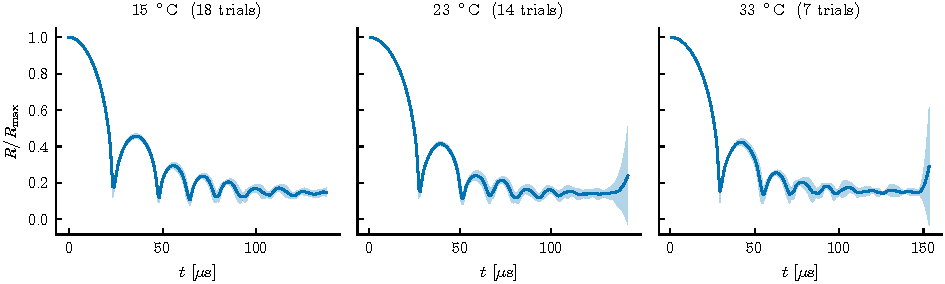
\includegraphics[width=\textwidth]{fig_records.pdf}
\caption{Measured records. Line is the mean over trials, band is $\pm$ one standard
deviation across trials at each time. The spread is the noise model.}
\label{fig:records}
\end{figure}

Two samples are excluded before fitting. A trial reading above its own maximum radius is
a tracking failure, and the $t=0$ sample where every trial agrees exactly is a definition
rather than a measurement --- giving it an error bar would invent an uncertainty and let
it constrain the fit.

Each candidate is evaluated on a log-spaced grid over its own parameters, at one
resolution for every model so that grid luck cannot decide the winner. The evidence is a
grid quadrature over that box, with the noise scale marginalised under a half-Cauchy
prior, a redundancy factor that down-weights parameters where a model merely reproduces a
simpler model it contains, and a BIC-style complexity penalty. Trajectories are
compressible (Keller--Miksis); the incompressible approximation changes the residuals by a
factor of two to four and must not be used for these records.

\section{Result}

Table~\ref{tab:fits} and Figure~\ref{fig:fits} give the outcome. The quadratic Zener model
\texttt{qSLS} --- strain-stiffening elasticity with stress relaxation --- wins at every
temperature, and the ordering beneath it separates cleanly into three tiers: models with
both ingredients, models with relaxation only, and memoryless models.

\begin{table}[htbp]
\centering
\caption{Best $\chi^2/N$ by model class. Values near $1$ indicate a fit within
experimental repeatability.}
\label{tab:fits}
\begin{tabular}{lccc}
\toprule
& \SI{15}{\celsius} & \SI{23}{\celsius} & \SI{33}{\celsius} \\
\midrule
\texttt{qSLS} (stiffening $+$ relaxation) & \textbf{1.35} & \textbf{1.33} & \textbf{1.23} \\
\texttt{SLS} (relaxation, linear elasticity) & 2.94 & 1.85 & 1.41 \\
viscoelastic fluids & 5.3--5.7 & 4.5--4.7 & 1.9--2.1 \\
memoryless & 12.6--16.7 & --- & --- \\
\bottomrule
\end{tabular}
\end{table}

\begin{figure}[htbp]
\centering
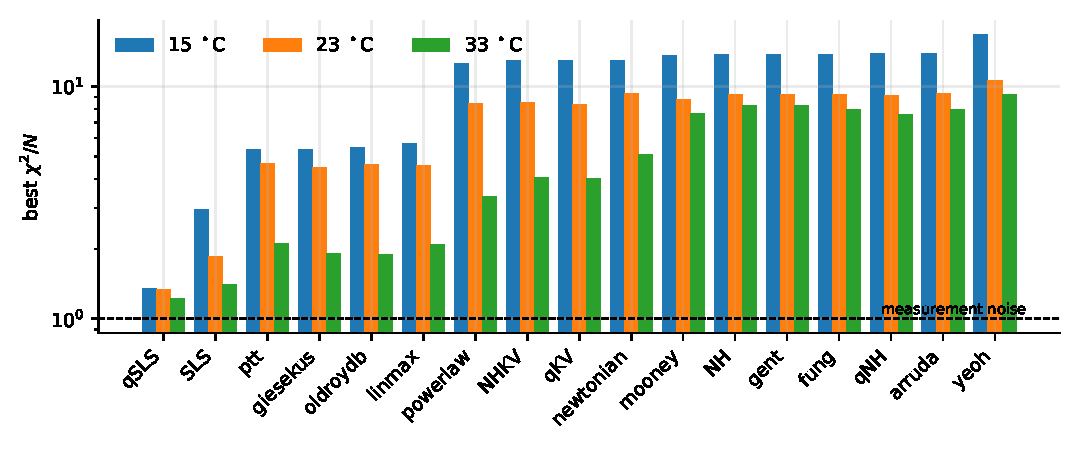
\includegraphics[width=\textwidth]{fig_fits.pdf}
\caption{Best $\chi^2/N$ for every candidate, all three temperatures, logarithmic scale.
The dashed line is the measurement-noise floor.}
\label{fig:fits}
\end{figure}

Figure~\ref{fig:winner} overlays the winning model on the data it was selected against.

\begin{figure}[htbp]
\centering
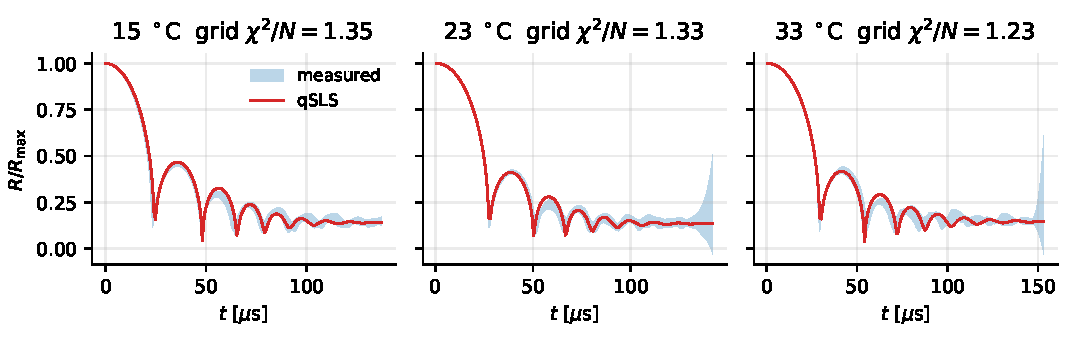
\includegraphics[width=\textwidth]{fig_winner.pdf}
\caption{The selected model against the measured band it was fitted to.}
\label{fig:winner}
\end{figure}

\subsection{Reading the posteriors}

The model posteriors saturate: the winner takes essentially all the mass and the
runners-up are reported as $10^{-29}$ or smaller. These magnitudes should not be read
literally. Evidence differences scale with sample count, and with roughly $3600$ samples a
modest per-sample difference in fit compounds into an astronomical Bayes factor. The
defensible reading is ordinal --- the winner is decisive and the ordering is meaningful,
the magnitudes are not. The residual $\chi^2/N$ is the quantity to quote.

\section{The temperature trend}

The most informative result is not any single number but a trend
(Figure~\ref{fig:trend}). The advantage that the stiffening term buys over pure relaxation
shrinks monotonically as the gel warms: the gap between \texttt{SLS} and \texttt{qSLS}
falls from $2.94$ versus $1.35$ at \SI{15}{\celsius} to $1.41$ versus $1.23$ at
\SI{33}{\celsius}. A warmer, softer gel needs less strain-stiffening to explain its
record. Because this is a trend across three independent datasets rather than a single
fitted value, it is harder to attribute to a fitting artefact than any individual
$\chi^2$.

\begin{figure}[htbp]
\centering
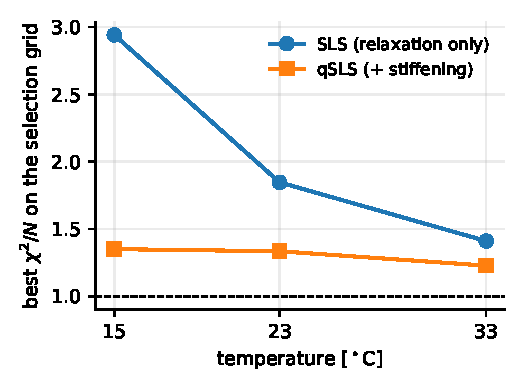
\includegraphics[width=0.5\textwidth]{fig_trend.pdf}
\caption{What the stiffening term buys, against temperature. The advantage of
\texttt{qSLS} over \texttt{SLS} narrows as the gel warms.}
\label{fig:trend}
\end{figure}

\section{Limitations}

\paragraph{The dropped points are outside the model, not outside the solver.}
Roughly one point in six of the winner's parameter box cannot be integrated. That is not a
numerical shortcoming. In that region the model expands to $R/R_0 = 2132$ after its
collapse --- identically at relative tolerances of $10^{-3}$, $10^{-4}$ and $10^{-5}$, so a
converged property of the equations rather than an artefact. The bubble begins at its
maximum radius and its energy is finite, so growth of that size is the constitutive model
failing, and refusing those points is the correct outcome.

The count of physically admissible points is pinned near $1958$ of $2401$ sampled whatever
the settings: looser tolerances and a $20\times$ step budget convert failures into runaways,
never into usable solves. This corrects an earlier reading of the same failures as a
stiffness problem. It also means the dropped points cannot be recovered by numerical
effort, and that no claim about the winner's fit should be made in that region.

\begin{figure}[htbp]
\centering
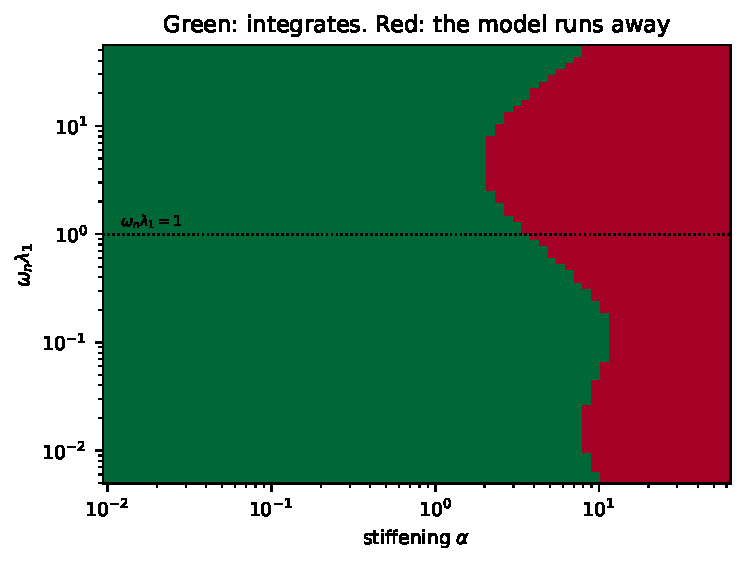
\includegraphics[width=0.58\textwidth]{fig_failure_map.pdf}
\caption{Where the winner can be integrated, at the fitted modulus and viscosity. Failure is
governed principally by the stiffening, and the threshold falls to its lowest where the
relaxation time is comparable to the bubble's own period --- but it is a boundary that moves,
not an isolated band.}
\label{fig:failure}
\end{figure}

\paragraph{The ranking survives; the parameter estimates do not.}
Independent sequential Monte Carlo runs give the winner $2173.55 \pm 0.19$ in log evidence
against $2071.90 \pm 0.38$ for the relaxation-only model --- a gap of $101.6$ against
run-to-run noise near $0.4$, so the comparison is resolved by a wide margin. The tensor grid
cannot say this on its own: it returns a single number with no uncertainty.

The same grid cannot estimate parameters. Refining it from $12$ to $20$ points per axis
moves the log evidence by $17.3$ and moves the best-fit point from $g = 658$, $\alpha = 1.52$
to $g = 144$, $\alpha = 8.86$, because the best cell is simply whichever node lands nearest
the ridge. Refinement cannot fix this: the posterior standard deviations are
$0.0018$, $0.0025$, $0.0055$ and $0.078$ in unit coordinates against a grid spacing of
$0.053$, so the posterior occupies about $10^{-7}$ of the prior volume and a uniform grid
would need of order $10^{10}$ points. Discretisation error of $17.3$ sits well inside the
$101.6$ gap, so the ranking is safe; the reported best-fit parameters are not.
Figure~\ref{fig:coverage} shows which models lose points.

\begin{figure}[htbp]
\centering
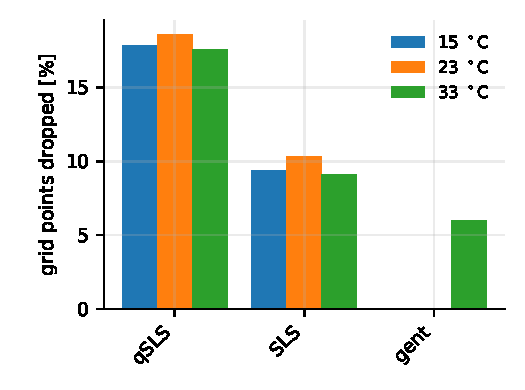
\includegraphics[width=0.5\textwidth]{fig_coverage.pdf}
\caption{Fraction of each model's parameter grid that could not be integrated. Models not
shown lost no points.}
\label{fig:coverage}
\end{figure}

\section{What the records determine, and what they do not}

The winner fits, but not every parameter it contains is measured by these data.

\subsection*{Why the trade exists}

Write $\hat g = G/p_\infty = 1/\mathrm{Ca}$ for the nondimensional modulus and
$\lambda = R_{\mathrm{eq}}/R$ for the stretch the stress law sees. The equilibrium stress
the Maxwell arm relaxes toward is
%
\begin{equation}
Z_e = R^3\left[\tfrac{3\alpha-1}{2}\,\hat g\,P(\lambda) + 2\alpha\,\hat g\,Q(\lambda)\right],
\qquad
\begin{aligned}
P(\lambda) &= 5 - \lambda^4 - 4\lambda,\\
Q(\lambda) &= \tfrac{27}{40} + \tfrac{1}{8}\lambda^8 + \tfrac{1}{5}\lambda^5 + \lambda^2 - \tfrac{2}{\lambda}.
\end{aligned}
\label{eq:Ze}
\end{equation}
%
Collecting powers of $\alpha$ separates it into two terms with different parameter
dependence,
%
\begin{equation}
Z_e = \hat g\,\alpha\,A(\lambda) + \hat g\,B(\lambda),
\qquad
A = R^3\!\left[\tfrac32 P + 2Q\right],
\qquad
B = -\tfrac12 R^3 P .
\label{eq:split}
\end{equation}
%
This is exact; it reproduces the implemented expression to $2.5\times10^{-14}$ over random
states. Only the first term carries $\alpha$, so $\hat g\alpha$ and $\hat g$ are separately
determined only while \emph{both} terms contribute.

They do not, at depth. As $\lambda$ grows, $Q \to \tfrac18\lambda^8$ dominates every other
term in either bracket, so $A \to \tfrac14 R^3\lambda^8$ while $B \sim \tfrac12 R^3\lambda^4$,
and
%
\begin{equation}
Z_e \;\longrightarrow\; \tfrac14\,\hat g\,\alpha\,R^3\lambda^8 ,
\end{equation}
%
a function of the \emph{product} $\hat g\alpha$ alone. The likelihood cannot then distinguish
a soft material that stiffens sharply from a stiff one that barely stiffens. Holding $Z_e$
fixed in~\eqref{eq:split} gives the trade in closed form,
%
\begin{equation}
\frac{\partial \log \hat g}{\partial \log \alpha}
= -\frac{\alpha A}{\alpha A + B}
\;\longrightarrow\; -1 \quad (\lambda \to \infty),
\label{eq:exponent}
\end{equation}
%
and the share of the signal that separates the two parameters is
%
\begin{equation}
\frac{|\hat g B|}{|\hat g \alpha A|} = \frac{|B|}{\alpha|A|} \simeq \frac{2}{\alpha\lambda^4}.
\label{eq:separability}
\end{equation}

Equations~\eqref{eq:exponent} and~\eqref{eq:separability} are what the measurements see.
These records collapse to $\lambda = 2.215$, where~\eqref{eq:exponent} gives $-0.981$ against
$-0.99$ from the Fisher curvature --- a prediction from the constitutive law, not a fit. The
profile likelihood returns $-0.80$ because it averages over a range of $\lambda$, and the
exponent is $-0.861$ at $\lambda = 1.5$. Separability falls as $\lambda^{-4}$: it is $2\%$ of
the signal at $\lambda = 2.2$ and $16\%$ at $\lambda = 1.5$.

\begin{figure}[htbp]
\centering
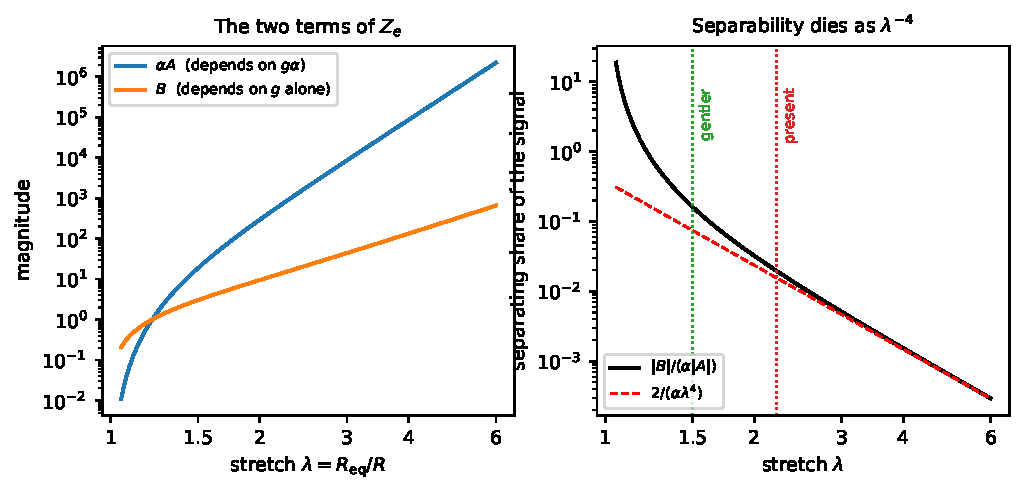
\includegraphics[width=0.98\textwidth]{fig_separability.pdf}
\caption{The two terms of~\eqref{eq:split} against collapse depth. Left: $\alpha A$, which
depends on the product $g\alpha$, outruns $B$, which carries $g$ alone. Right: their ratio,
the share of the signal that can separate the two parameters, following
$2/(\alpha\lambda^4)$ once the collapse is deep. It is $2\%$ at the depth these records
reach and $16\%$ at $\lambda = 1.5$.}
\label{fig:separability}
\end{figure}

\subsection*{What the Fisher information measures}

For Gaussian observations with known deviations the log-likelihood is
$-\tfrac12\sum_i (y_i - m_i(\theta))^2/\sigma_i^2$ up to a constant, so with the whitened
sensitivity $J_{ij} = \sigma_i^{-1}\partial m_i/\partial\theta_j$ the Fisher information is
exactly $F = J^{\mathsf T}J$, and $\Delta\chi^2 \simeq \Delta\theta^{\mathsf T} F \Delta\theta$.
Taking $\theta$ to be the logarithms of the parameters makes the eigenvectors read as
power-law combinations: along an eigenvector $v$ the ratio $v_g/v_\alpha$ is the exponent
in $g \propto \alpha^{v_g/v_\alpha}$. This is also the observability Gramian of the system
augmented with $\dot\theta = 0$, which is why identifiability and observability are the same
statement here.

One caution, since it caught us. When the sensitivities are taken with respect to a unit
cube $u_j = (\log\theta_j - a_j)/w_j$ rather than $\log\theta_j$ directly, the eigenvector
components carry the box widths: $\Delta\log\theta_j = w_j\,\tilde v_j$, so the exponent is
$(w_g \tilde v_g)/(w_\alpha \tilde v_\alpha)$, not $\tilde v_g/\tilde v_\alpha$. With $w$ of
three and four decades the two differ by $25\%$.

\begin{figure}[htbp]
\centering
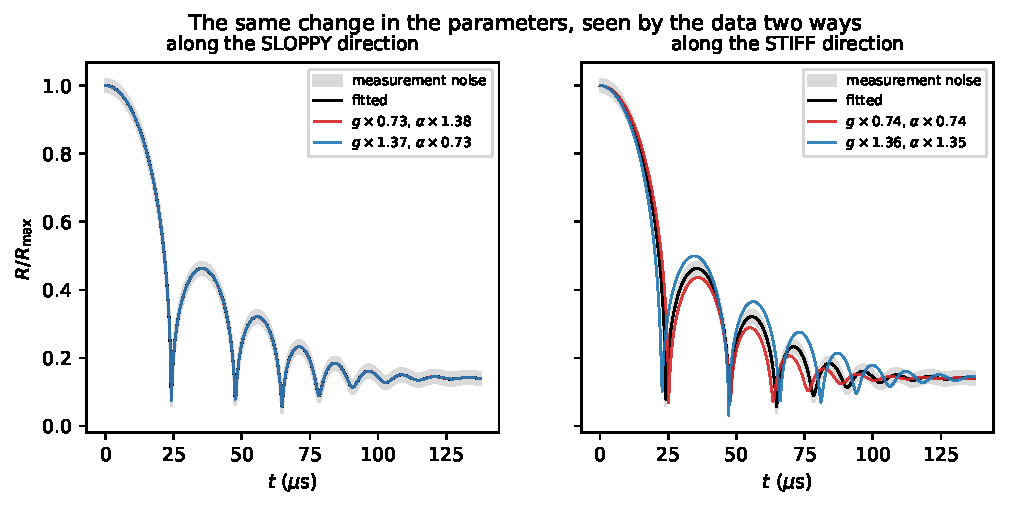
\includegraphics[width=0.98\textwidth]{fig_eigenvectors.pdf}
\caption{What an eigenvector means, shown rather than defined. The parameters are moved the
same distance in $\log$-space along each eigenvector. Along the sloppy direction a $27\%$
change in the modulus, compensated by $38\%$ in the stiffening, leaves the trajectory inside
the measurement noise; along the stiff direction a change of the same size is obvious. The
data cannot see the first and cannot miss the second.}
\label{fig:eigenvectors}
\end{figure}

\begin{figure}[htbp]
\centering
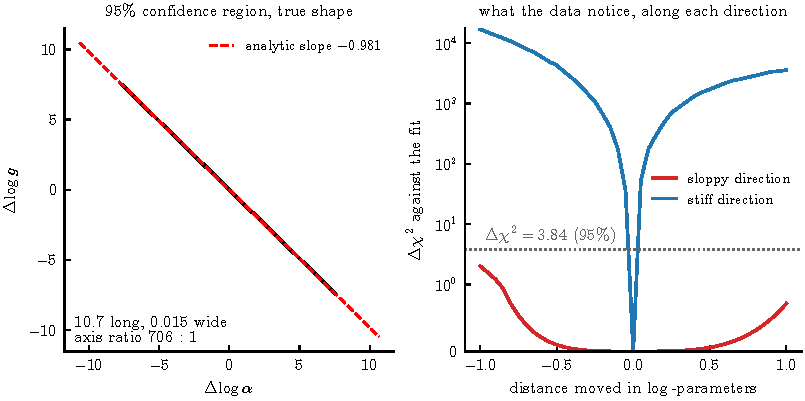
\includegraphics[width=0.98\textwidth]{fig_ellipse.pdf}
\caption{Left: the $95\%$ region from the inverse Fisher information, $10.7$ long and
$0.015$ wide in $\log$-parameters --- an axis ratio of $706$, which is why it draws as a
line, and the analytic slope of $-0.981$ lies along it. Right: the misfit measured by
re-solving at perturbed parameters, not the quadratic approximation. Moving along the stiff
direction costs $10^4$ in $\Delta\chi^2$; moving the same distance along the sloppy one stays
below the $95\%$ threshold, so the parameters may shift by a factor of $e \approx 2.7$
without the data objecting.}
\label{fig:ellipse}
\end{figure}

\subsection*{Designing without assuming the model}

Everything above optimises the Fisher information of one model at its fitted parameters,
which is circular if that model is wrong. Two checks that do not privilege it.

\paragraph{The record is information-rich; the parameterisation is not.}
Drawing $400$ trajectories from the posterior and taking the singular values of the centred
ensemble, eleven modes rise above the trial noise floor of $0.018\,R_{\max}$. That is not a
count of identifiable combinations --- four varied parameters span at most a four
dimensional manifold, and the extra modes are its curvature --- but it does say the
measurement can distinguish far more shapes than the fit extracts. The limit is how qSLS
parameterises the physics, not the information in the record.

\paragraph{Discrimination does not privilege a model.}
T-optimality (Atkinson and Fedorov, \emph{Biometrika} \textbf{62}, 1975) asks a different question: which design makes the
candidates disagree most? Root-mean-square separation between predictions at each model's
own fit, in units of the measurement noise:

\begin{center}
\begin{tabular}{lccc}
\toprule
design & qSLS--SLS & qSLS--qKV & qSLS--NHKV \\
\midrule
$277\,\mu$m, stretch $7.09$ (present) & $2.69$ & $4.92$ & $5.91$ \\
$277\,\mu$m, stretch $5.00$ & $5.06$ & $6.78$ & $7.65$ \\
$277\,\mu$m, stretch $3.00$ & $5.46$ & $7.51$ & $9.96$ \\
$895\,\mu$m, stretch $4.93$ & $\mathbf{8.08}$ & $8.13$ & $8.55$ \\
$100\,\mu$m, stretch $20.0$ & $6.62$ & $8.93$ & $9.19$ \\
\bottomrule
\end{tabular}
\end{center}

The present design is the weakest in the set at separating the candidates: qSLS and SLS
differ by $2.7$ noise units where a gentler collapse gives $5.1$ and a larger, gentler one
gives $8.1$.

This matters because the two objectives share no assumptions. One maximises precision
\emph{within} qSLS and presumes it correct; the other measures divergence \emph{between}
models and presumes none of them. They point the same way. That agreement is stronger
evidence for the recommendation than either alone, and it is the answer to the obvious
objection that a model-specific design criterion cannot justify itself.

Where they differ is which gain to prefer. Conditioning within qSLS favours the present
bubble size at a gentler collapse; discrimination favours a larger bubble as well. Since the
residual analysis says the model is missing structure, discrimination is the more defensible
priority, and that argues for the larger bubble.

\subsection*{Why the design criteria disagree}

The classical criteria are all functionals of the same $F$: $\det F$ (D), $\operatorname{tr}
F^{-1}$ (A), $\lambda_{\min}$ (E), and $c^{\mathsf T}F^{-1}c$ for one combination (c). A
design change that merely amplifies the signal --- a larger bubble, a longer record, less
noise --- multiplies $F$ by a scalar $s$. Then $\lambda_{\min} \to s\lambda_{\min}$ and
$\det F \to s^p \det F$, so D and E both improve, while
%
\begin{equation}
\kappa = \lambda_{\max}/\lambda_{\min}
\end{equation}
%
is unchanged. Degeneracy is a property of the \emph{directions}, and only a design that
alters them can fix it. That is why the E-optimal search preferred a larger bubble
($895\,\mu$m, $\lambda_{\min} = 12.8$) while the conditioning and the eigenvector
composition preferred a gentler collapse at the present size ($277\,\mu$m at stretch $5$,
$\kappa = 4.2\times10^3$, and the modulus-stiffening share of the worst direction falling
from $87\%$ to $66\%$). Both are correct answers to different questions, and
\eqref{eq:separability} says which question matters here.

\paragraph{Modulus and stiffening trade against each other.}
Two independent analyses agree. The Fisher information at the fitted optimum has an
eigenvalue spectrum spanning six decades, and the eigenvector of its smallest eigenvalue is
almost purely a shear-modulus-against-stiffening direction, with weights $-0.796$ and
$+0.604$ and contributions of $-0.003$ and $-0.032$ from viscosity and relaxation time.
Separately, profiling the likelihood in $\alpha$ --- fixing it and re-optimising everything
else --- gives $g \propto \alpha^{-0.80}$ across two decades. Sampling the posterior gives a
third, independent measurement: its widest direction is
$(-0.682,\,+0.002,\,-0.082,\,+0.727)$ in the logarithms of
$(g, \mu, \lambda_1, \alpha)$, and $\log g$ is $98.7\%$ anticorrelated with $\log\alpha$.

The three exponents are $-0.99$ from local curvature, $-0.94$ from the posterior covariance,
and $-0.80$ from the profile. They agree that the trade is near-reciprocal and disagree in
the third digit, which is expected rather than troubling: the valley is curved, so a
curvature estimate at one point and a chord measured across two decades are not measuring
the same slope. The correlation is the more robust statement.

So viscosity and relaxation time are cleanly determined, while modulus and stiffening are
constrained only in combination. The identifiable quantity is closer to $g\,\alpha^{0.8}$
than to either alone, and a fitted $\alpha$ should be reported with its correlation to $g$
rather than as an independent material property.

\begin{figure}[htbp]
\centering
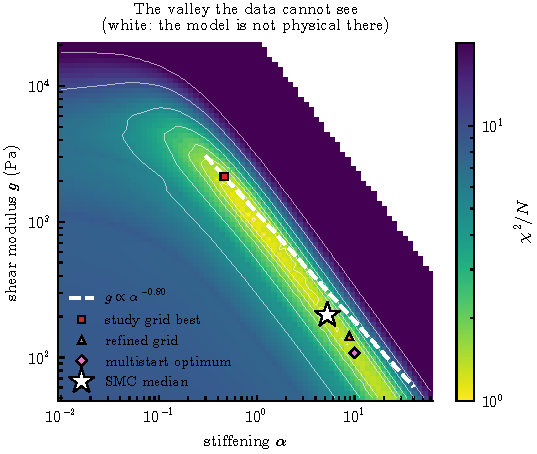
\includegraphics[width=0.62\textwidth]{fig_valley.pdf}
\caption{$\chi^2/N$ over the modulus--stiffening plane, at the fitted viscosity and
relaxation time. The dashed line is $g \propto \alpha^{-0.80}$, predicted from the Fisher
curvature at a single point; it lies along the floor of the valley. Four ``best fits'' from
four methods are strung out along that floor rather than disagreeing with one another. The
white region at upper right is where the model is not physical.}
\label{fig:valley}
\end{figure}

Figure~\ref{fig:valley} shows why the four estimates in this study disagree about $g$ by an
order of magnitude while agreeing about the fit: they are different points on the floor of a
single flat-bottomed trench.

\paragraph{The stiffening is nonetheless identified, once the prior allows it.}
Sampling with the ceiling on $\alpha$ placed at $1$, $10$ and $100$:

\begin{center}
\begin{tabular}{cccc}
\toprule
ceiling & log evidence & median $\alpha$ & $97.5\%$ \\
\midrule
$1$ & $2162.9$ & $0.85$ & $0.97$ \\
$10$ & $2173.9$ & $6.37$ & $9.04$ \\
$100$ & $2172.4$ & $5.27$ & $8.73$ \\
\bottomrule
\end{tabular}
\end{center}

Widening the prior tenfold moves the median only from $6.37$ to $5.27$ and the evidence by
$1.5$ out of $2173$, so $\alpha$ is identified near $5$ with $97.5\%$ of posterior mass
below about $9$. A prior-dominated parameter would have tracked its bound. The ceiling of
$1$ shows what genuine truncation looks like: the median pins against it and $11$ log units
of evidence are lost.

This corrects a natural reading of the profile likelihood alone, which appears flat to the
boundary only because the boundary sits where the posterior's upper tail does.

\begin{figure}[htbp]
\centering
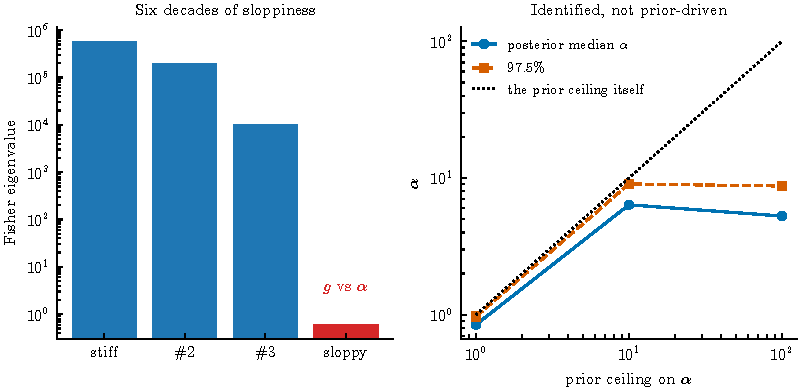
\includegraphics[width=0.98\textwidth]{fig_identifiability.pdf}
\caption{Left: the Fisher spectrum at the optimum, six decades between the stiffest and
sloppiest directions, with the sloppiest being modulus against stiffening. Right: the
posterior for $\alpha$ against the ceiling imposed on its prior. It tracks the ceiling while
truncated and departs from it once the ceiling is loose, which is what distinguishes an
identified parameter from a prior-driven one.}
\label{fig:identifiability}
\end{figure}

\paragraph{Consequences for the numbers reported here.}
Three methods that resolve the posterior --- sampling, a refined grid, and continuous
optimisation --- agree that $g$ lies near $10^2$\,Pa. The coarse grid used for the ranking
reports $2154$\,Pa. The ranking does not depend on this, but any material property quoted
from the grid does. We also note that a modulus of that size is implausibly soft for
gelatin, which is the degeneracy above making itself felt: the fit buys a lower residual by
trading modulus against stiffening, along a direction the data barely constrain.

\paragraph{One candidate was never genuinely exercised.}
The Gent solid appears in the comparison but cannot be tested on these records. Its energy
diverges as $I_1 - 3 \to J_m$, and a Gent solid soft enough to be distinguishable from
Neo-Hookean predicts a collapse it cannot sustain, so it locks up. Where it does
integrate, it differs from Neo-Hookean by $1.7\times10^{-4}$ of $R_{\max}$ against
measurement noise near $2\times10^{-2}$ --- two orders of magnitude below what the data can
resolve. Any statement about strain-stiffening laws here excludes it.

\paragraph{The noise model sees only repeatability.}
Using trial-to-trial spread as the noise means $\chi^2/N \approx 1$ certifies agreement to
within experimental repeatability. A systematic error common to every trial would not
appear in that spread, and would show up instead as exactly the kind of residual excess we
report --- $20$ to $35\%$ above the noise floor. This study cannot separate that from
genuine model inadequacy.

\section{Reproducing}

\begin{verbatim}
.venv/bin/python examples/measured_selection.py <dataset> [thermal Nt] [workers]
.venv/bin/python docs/writeup/collect.py 16     # records results.json
.venv/bin/python docs/writeup/figures.py        # draws every figure from it
\end{verbatim}

Every number and figure in this document comes from \texttt{results.json}; none is
transcribed by hand.

\end{document}
